\documentclass[11pt]{article}
\usepackage[margin=1in]{geometry}
\usepackage{graphicx}
\usepackage{amsmath,amssymb}
\usepackage{tikz}

\usepackage{pgfplots}
\usepackage{titlesec}
\usepackage{url}
\usepackage{verbatim}
\usepackage{hyperref}
\usetikzlibrary{calc}
\graphicspath{{../Screenshots/}}

% compact spacing
\setlength{\parskip}{6pt}
\setlength{\parindent}{0pt}

% Draw solid square with side label b (size is parameter in cm)
\newcommand{\DrawSolidBox}[1]{%
  \begin{tikzpicture}[scale=#1]
    \draw[line width=0.6pt] (0,0) rectangle (3,3);
    \draw[<->,line width=0.5pt]
      (0,1.5) -- node[above] {$b$} (3,1.5);
  \end{tikzpicture}%
}

% Hollow square with separated arrows
\newcommand{\DrawHollowBox}[2]{%
  % #1 = scale, #2 = gamma
  \begin{tikzpicture}[scale=#1]
    \def\L{3}%
    \pgfmathsetmacro{\g}{#2}
    \pgfmathsetmacro{\inset}{(3-3*\g)/2}
    \draw[line width=0.6pt] (0,0) rectangle (\L,\L);
    \draw[line width=0.6pt]
      (\inset,\inset) rectangle (\inset+3*\g,\inset+3*\g);

    % Outer b arrow slightly above center (y = 1.95)
    \draw[<->,line width=0.5pt]
      (0,1.95) -- node[above] {$b$} (3,1.95);

    % Inner gamma b arrow slightly below center (y = 1.05)
    \draw[<->,line width=0.5pt]
      (\inset,1.05) --
      node[below] {$\gamma b$}
      (\inset+3*\g,1.05);
  \end{tikzpicture}%
}



\begin{document}
\section{MSDS: Materials Safety Data Sheets}
\begin{enumerate}
    \item standard documents that provide safety info on Materials
    \item provided by suppliers
    \item include info on:
    \begin{itemize}
        \item composition
        \item handling + PPE (Personal protective equipment)
        \item hazards
        \item shipping regulations
    \end{itemize}
\end{enumerate}
\section{Legislation}
\begin{itemize}
    \item can support all 3 capitals
    \item includes state, national, and internation standards+agreements
\end{itemize}
\section{EV case study}
People:
\begin{itemize}
    \item range anxiety
    \item 
\end{itemize}
Planet:
\begin{itemize}
    \item Concerns over the carbon emission of energy grid
    \item are carbon emissions better for EVs?
    \item legislation in EU requires battery recycling
\end{itemize}
Prosperity:
\begin{itemize}
    \item Li only produced by 2 major countries
    \item current Li production does not meet anticipated demand
    \item Nd production too low
    \item 95\% of Nd from one country(China)
\end{itemize}









































\newpage
\begin{center}
\begin{minipage}[t]{0.47\textwidth}
\centering
\DrawSolidBox{0.9}

\smallskip
$A_s$ (solid square)
\end{minipage}\hfill
\begin{minipage}[t]{0.47\textwidth}
\centering
\DrawHollowBox{0.9}{0.55}

\smallskip
$A_h$ (hollow square)
\end{minipage}
\end{center}
% Objective: maximize EI for a thin-walled square tube
\textbf{Objective:} Maximize \(EI\)

\[
A_s = b^2
\]

\[
A_{\text{gap}} = (b-2t)^2 \quad \text{where } t \text{ is thickness}
\]

Thin-wall assumption: \(t \ll b\)

\[
A_s - A_g = A_h = 4 b t
\]

Expanding \(I\):
\[
I = I_s - I_{\text{gap}}
   = \frac{b^4}{12} - \frac{(b-2t)^4}{12}
   = \frac{A_s^{\,2} - A_{\text{gap}}^{\,2}}{12}
   = \frac{(A_s - A_g)(A_s + A_g)}{12}
\]

\[
I = \frac{[4 b t]\left(b^2 + (b-2t)^2\right)}{12}
  = \frac{8 b^3 t - 16 b^2 t^2 + 16 b t^3}{12}
\]

By the thin-wall assumption: \(b t^3,\; b^2 t^2 \ll b^3 t\)

\[
I \approx \frac{2}{3} b^3 t
\]

Mass constraint:
\[
m = 4 b t \rho L \quad \Rightarrow \quad
t = \frac{m}{4 b \rho L}
\]

Hence
\[
I \approx \frac{2}{3} b^3 \!\left(\frac{m}{4 b \rho L}\right)
= \frac{1}{6}\, \frac{m\, b^2}{\rho L}
\]

Back to the objective:
\[
E\!I \approx E \left(\frac{2}{3} b^3\right)\!\left(\frac{m}{4 b \rho L}\right)
\]

Define the material index
\[
M=\frac{E}{\rho}
\]

Taking logs for selection charts:
\[
\log E = \log \rho + \log M
\]
\begin{center}
    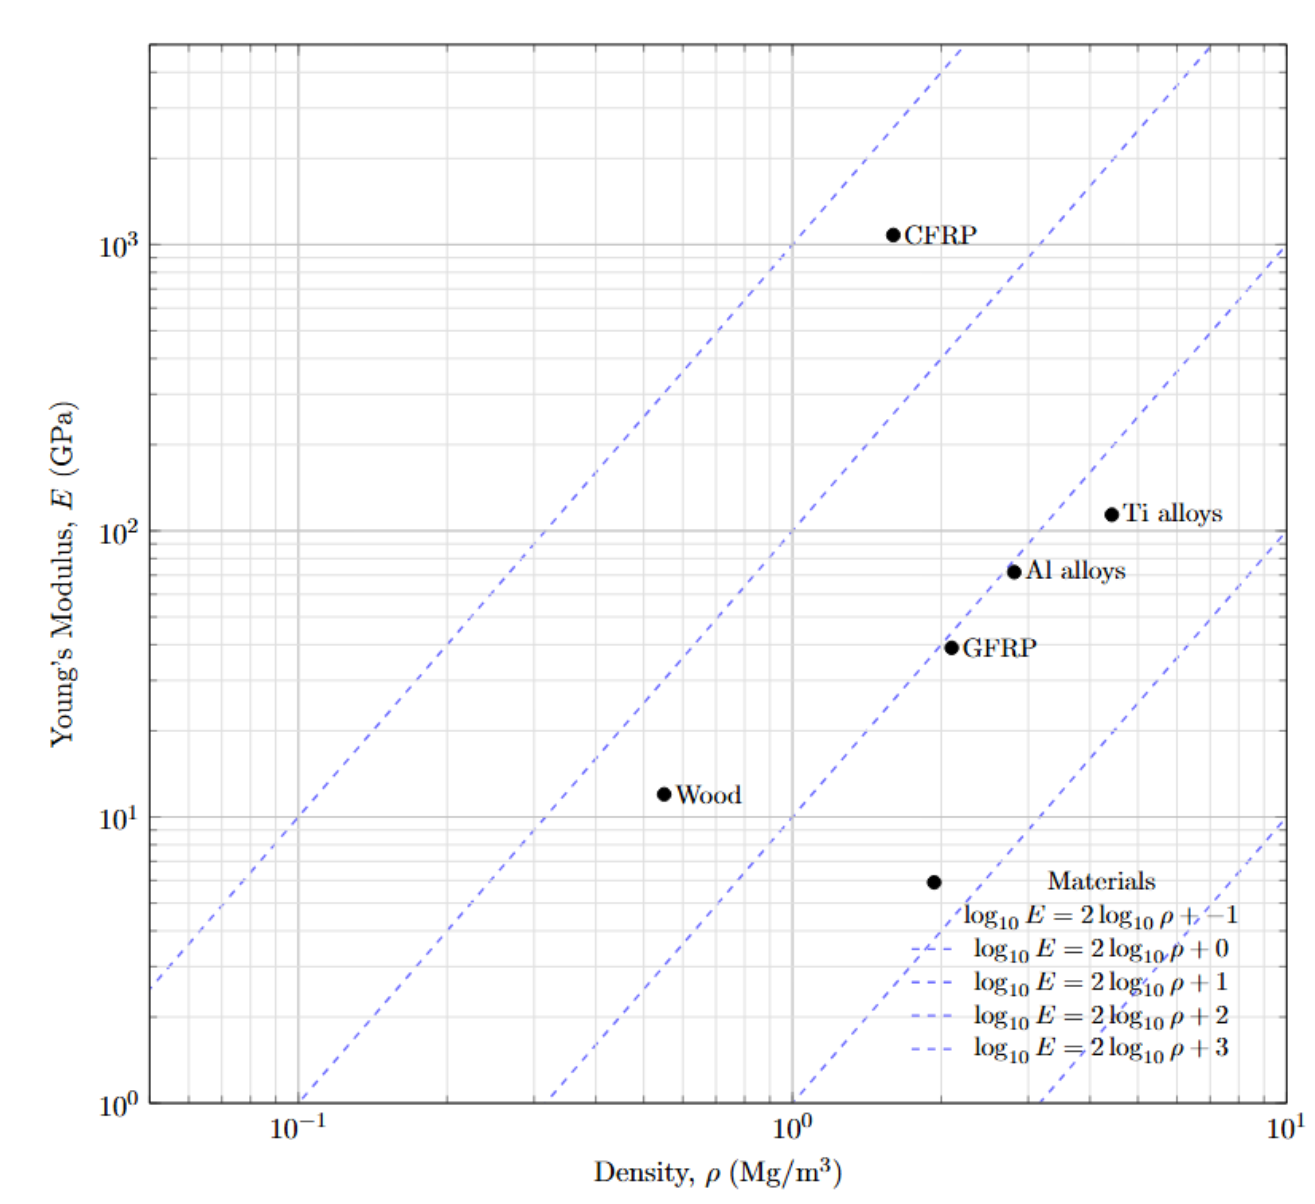
\includegraphics[width = 250pt]{Screenshot 2025-12-01 173111.png}
\end{center}
\url{https://hal.science/jpa-00251707/document}
\end{document}